\documentclass{standalone}% For the example only, any class will do

\usepackage{tikz}

\begin{document}
\tikzset{every picture/.style={line width=0.75pt}} %set default line width to 0.75pt

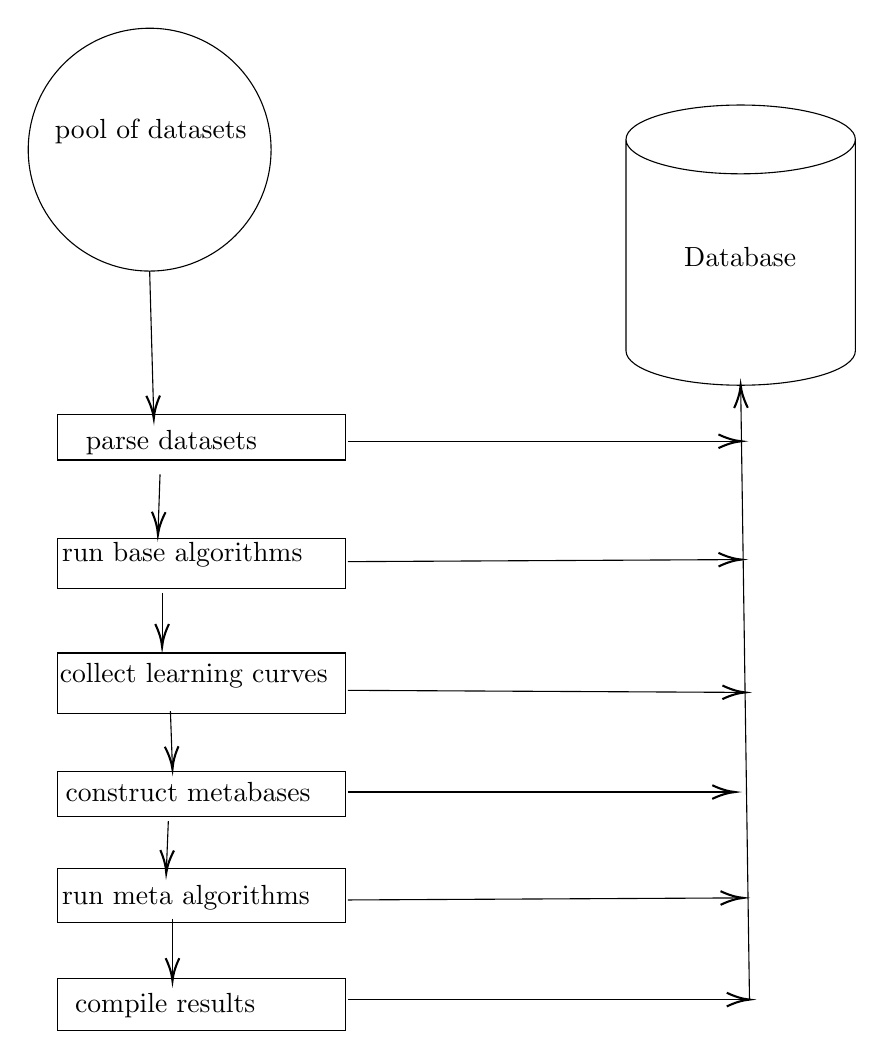
\begin{tikzpicture}[x=0.75pt,y=0.75pt,yscale=-1,xscale=1]
%uncomment if require: \path (0,491); %set diagram left start at 0, and has height of 491

%Shape: Circle [id:dp5066955303041745]
\draw   (16,61.5) .. controls (16,29.19) and (42.19,3) .. (74.5,3) .. controls (106.81,3) and (133,29.19) .. (133,61.5) .. controls (133,93.81) and (106.81,120) .. (74.5,120) .. controls (42.19,120) and (16,93.81) .. (16,61.5) -- cycle ;
%Straight Lines [id:da4328641283769663]
\draw    (74.5,120) -- (76.44,189) ;
\draw [shift={(76.5,191)}, rotate = 268.39] [color={rgb, 255:red, 0; green, 0; blue, 0 }  ][line width=0.75]    (10.93,-3.29) .. controls (6.95,-1.4) and (3.31,-0.3) .. (0,0) .. controls (3.31,0.3) and (6.95,1.4) .. (10.93,3.29)   ;

%Shape: Rectangle [id:dp11150860688027087]
\draw   (30,189) -- (169,189) -- (169,211) -- (30,211) -- cycle ;
%Shape: Rectangle [id:dp9239719015341326]
\draw   (30,249) -- (169,249) -- (169,273) -- (30,273) -- cycle ;
%Shape: Rectangle [id:dp5977052266732532]
\draw   (30,304) -- (169,304) -- (169,333) -- (30,333) -- cycle ;
%Shape: Rectangle [id:dp9893498709782924]
\draw   (30,361) -- (169,361) -- (169,383) -- (30,383) -- cycle ;
%Shape: Rectangle [id:dp28178812250160634]
\draw   (30,408) -- (169,408) -- (169,434) -- (30,434) -- cycle ;
%Shape: Rectangle [id:dp5802215180629449]
\draw   (30,461) -- (169,461) -- (169,486) -- (30,486) -- cycle ;
%Straight Lines [id:da05648979970272139]
\draw    (79.5,218) -- (78.57,245) ;
\draw [shift={(78.5,247)}, rotate = 271.97] [color={rgb, 255:red, 0; green, 0; blue, 0 }  ][line width=0.75]    (10.93,-3.29) .. controls (6.95,-1.4) and (3.31,-0.3) .. (0,0) .. controls (3.31,0.3) and (6.95,1.4) .. (10.93,3.29)   ;

%Straight Lines [id:da2175210199156956]
\draw    (80.5,275) -- (80.5,299) ;
\draw [shift={(80.5,301)}, rotate = 270] [color={rgb, 255:red, 0; green, 0; blue, 0 }  ][line width=0.75]    (10.93,-3.29) .. controls (6.95,-1.4) and (3.31,-0.3) .. (0,0) .. controls (3.31,0.3) and (6.95,1.4) .. (10.93,3.29)   ;

%Straight Lines [id:da010709021104718719]
\draw    (84.5,332) -- (85.43,358) ;
\draw [shift={(85.5,360)}, rotate = 267.95] [color={rgb, 255:red, 0; green, 0; blue, 0 }  ][line width=0.75]    (10.93,-3.29) .. controls (6.95,-1.4) and (3.31,-0.3) .. (0,0) .. controls (3.31,0.3) and (6.95,1.4) .. (10.93,3.29)   ;

%Straight Lines [id:da7311987759547272]
\draw    (83.5,385) -- (82.58,408) ;
\draw [shift={(82.5,410)}, rotate = 272.29] [color={rgb, 255:red, 0; green, 0; blue, 0 }  ][line width=0.75]    (10.93,-3.29) .. controls (6.95,-1.4) and (3.31,-0.3) .. (0,0) .. controls (3.31,0.3) and (6.95,1.4) .. (10.93,3.29)   ;

%Straight Lines [id:da08959142481397442]
\draw    (85.5,432) -- (85.5,460) ;
\draw [shift={(85.5,462)}, rotate = 270] [color={rgb, 255:red, 0; green, 0; blue, 0 }  ][line width=0.75]    (10.93,-3.29) .. controls (6.95,-1.4) and (3.31,-0.3) .. (0,0) .. controls (3.31,0.3) and (6.95,1.4) .. (10.93,3.29)   ;

%Shape: Can [id:dp11787917120483149]
\draw   (414.5,56.58) -- (414.5,158.43) .. controls (414.5,167.58) and (389.76,175) .. (359.25,175) .. controls (328.74,175) and (304,167.58) .. (304,158.43) -- (304,56.58)(414.5,56.58) .. controls (414.5,65.73) and (389.76,73.15) .. (359.25,73.15) .. controls (328.74,73.15) and (304,65.73) .. (304,56.58) .. controls (304,47.42) and (328.74,40) .. (359.25,40) .. controls (389.76,40) and (414.5,47.42) .. (414.5,56.58) -- cycle ;
%Straight Lines [id:da6414966827229298]
\draw    (363.5,471) -- (359.28,177) ;
\draw [shift={(359.25,175)}, rotate = 449.18] [color={rgb, 255:red, 0; green, 0; blue, 0 }  ][line width=0.75]    (10.93,-3.29) .. controls (6.95,-1.4) and (3.31,-0.3) .. (0,0) .. controls (3.31,0.3) and (6.95,1.4) .. (10.93,3.29)   ;

%Straight Lines [id:da7660502953112669]
\draw    (170,202) -- (357.5,202) ;
\draw [shift={(359.5,202)}, rotate = 180] [color={rgb, 255:red, 0; green, 0; blue, 0 }  ][line width=0.75]    (10.93,-3.29) .. controls (6.95,-1.4) and (3.31,-0.3) .. (0,0) .. controls (3.31,0.3) and (6.95,1.4) .. (10.93,3.29)   ;

%Straight Lines [id:da4531781376733226]
\draw    (170,260) -- (357.5,259.01) ;
\draw [shift={(359.5,259)}, rotate = 539.71] [color={rgb, 255:red, 0; green, 0; blue, 0 }  ][line width=0.75]    (10.93,-3.29) .. controls (6.95,-1.4) and (3.31,-0.3) .. (0,0) .. controls (3.31,0.3) and (6.95,1.4) .. (10.93,3.29)   ;

%Straight Lines [id:da49812827508731594]
\draw    (170,322) -- (359.38,322.99) ;
\draw [shift={(361.38,323)}, rotate = 180.3] [color={rgb, 255:red, 0; green, 0; blue, 0 }  ][line width=0.75]    (10.93,-3.29) .. controls (6.95,-1.4) and (3.31,-0.3) .. (0,0) .. controls (3.31,0.3) and (6.95,1.4) .. (10.93,3.29)   ;

%Straight Lines [id:da7940516102035275]
\draw    (170,371) -- (354.5,371) ;
\draw [shift={(356.5,371)}, rotate = 180] [color={rgb, 255:red, 0; green, 0; blue, 0 }  ][line width=0.75]    (10.93,-3.29) .. controls (6.95,-1.4) and (3.31,-0.3) .. (0,0) .. controls (3.31,0.3) and (6.95,1.4) .. (10.93,3.29)   ;

%Straight Lines [id:da043855488461804315]
\draw    (170,423) -- (358.5,422.01) ;
\draw [shift={(360.5,422)}, rotate = 539.72] [color={rgb, 255:red, 0; green, 0; blue, 0 }  ][line width=0.75]    (10.93,-3.29) .. controls (6.95,-1.4) and (3.31,-0.3) .. (0,0) .. controls (3.31,0.3) and (6.95,1.4) .. (10.93,3.29)   ;

%Straight Lines [id:da8355322171480093]
\draw    (170,471) -- (361.5,471) ;
\draw [shift={(363.5,471)}, rotate = 180] [color={rgb, 255:red, 0; green, 0; blue, 0 }  ][line width=0.75]    (10.93,-3.29) .. controls (6.95,-1.4) and (3.31,-0.3) .. (0,0) .. controls (3.31,0.3) and (6.95,1.4) .. (10.93,3.29)   ;


% Text Node
\draw (75,53) node  [align=left] {pool of datasets};
% Text Node
\draw (85,202.5) node  [align=left] {parse datasets};
% Text Node
\draw (90.25,256.5) node  [align=left] {run base algorithms};
% Text Node
\draw (95.75,315) node  [align=left] {collect learning curves};
% Text Node
\draw (93,371) node  [align=left] {construct metabases};
% Text Node
\draw (92,422) node  [align=left] {run meta algorithms};
% Text Node
\draw (82,474) node  [align=left] {compile results};
% Text Node
\draw (359,113) node  [align=left] {Database};


\end{tikzpicture}
\end{document}
